\documentclass[a4paper 12pts]{article}
\usepackage[utf8]{inputenc}
\usepackage[T1]{fontenc}
\usepackage[francais]{babel}
\usepackage{graphicx}


\title{Rapport de Projet : iRover}

%mettez vos noms svp !!

\author{R. Joachim CLAYTON, Geoffrey DESBROSSES, Clément BAUCHET, }

\begin{document}

\maketitle


\begin{figure}[h]
   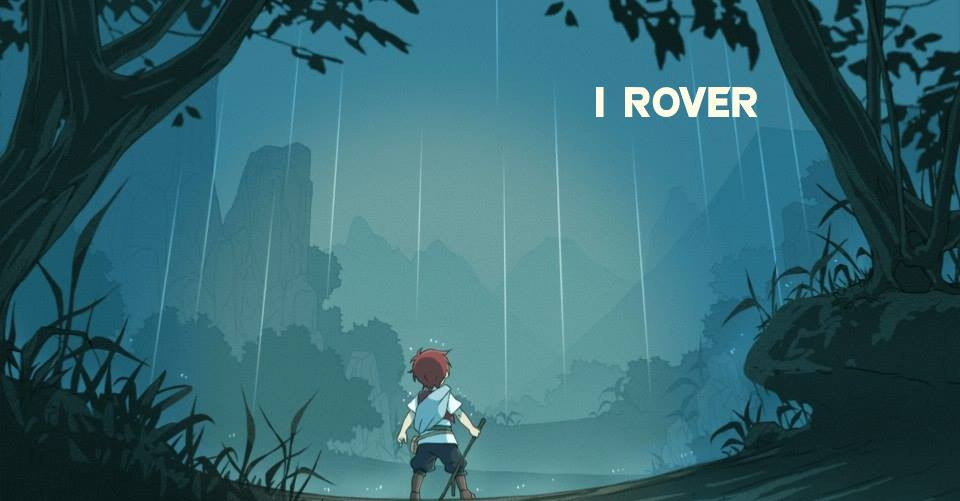
\includegraphics[width=350pt]{Illustration/proj_irover.jpg}
	\caption{iRover, l'histoire d'un héros qu'on appellait robot}
\end{figure}



\newpage


\renewcommand{\contentsname}{Sommaire} 
\tableofcontents

\newpage








\section{Rapport de Projet}


\vspace{2cm}



\subsection{Introduction}

Le projet a pour objectif la création d'une application graphique où un petit personnage (robot) réaliserait une tache particulière.\\
Pour cela nous avons imaginé un scénario de mini jeu semblable au jeux en deux dimensions où notre robot prendrait la forme d'un héros sans peur et sans reproche.\\
L'autre aspect de ce projet est de pousser notre groupe à utiliser, comprendre et intégrer les autotools à savoir : 

\begin{enumerate}
\item Utilisation des autotools.
\item Génération d'une documentation technique avec Doxygen.
\item Utilisation d'une platforme svn pour la réalisation de notre projet.
\item Rédaction de documents avec \LaTeX .
\item Réalisation de quelques test avec cppedit.

\end{enumerate}

\vspace{075 cm}

\subsection{Membre du groupe et tâches de chacun}


\begin{tabbing}
Voici \= un petit exemple \= de l'environnement tabbing \\
\> on commence au premier repère \\
\> \> ici on est au second repère
\end{tabbing}

\vspace{1 cm}

\begin{tabbing}

\hspace{4cm} \= \hspace{6cm} \= \hspace{2cm} \= \kill
\textbf{Responsable} \> \textbf{Tâche} \> \textbf {Description} \\
\\
Clément Bauchet \> Création graphique \> La création de l'environnement \\
 \> \>graphiques et des images \\					
\> Parsing de la carte \>L'interprétation entre les objets \\
\> \> graphiques et les objets C++\\					
\\
Geoffrey Desbrosses \> Création des objets \> Création de chaque objet de l'application\\
\> \> et de leurs actions\\
\> Documentation du code source \> Gestion de la documentation Doxygen \\ 
\\
\> IHM \> Interface utilisateur de l'application. \> \\
\\
Jean-Christophe Guerin \> IA  \> Définitions des algorithmes de pathfinding\\
\> \> de déplacement et de découverte\\	
\\
Joachim Clayton \> Documentation utilisateur \> Redaction de la documentation utilisateur \\
\\ 
\end{tabbing}


\newpage

\section{Définition de la carte}
\vspace{1cm}
Pour commencer, il fallait générer un ou plusieurs terrains à l'aide du logiciel \emph{Tiled}, un éditeur de cartes. La carte est créée avec une certaine tilesheet (une image contenant le dessin de toutes les cases possibles), et enregistrée sous le format \textbf{.tmx}, un format de type XML.

Pour pouvoir afficher le terrain dans notre application, nous avons d'abord fait appel au module \emph{ClanXML} de la bibliothèque \emph{ClanLib} qui est utilisée pour notre application, notamment pour l'affichage. Une classe \textbf{Map} a été créée, représentant le terrain et ses informations : les dimensions, les types de ses cases et la praticabilité de celles-ci par le robot ou d'autres entités. A la création d'une carte, ces informations sont récupérées directement depuis le fichier de carte .tmx fourni, en le parsant en tant que document DOM comme permis par \emph{ClanXML}. \\
\emph{N.B. :} A l'heure actuelle, il n'est pas possible de déterminer par seule lecture du fichier .tmx quels types de cases sont praticables par le robot. Ceci est déterminé au cas par cas dans le code. De plus, la praticabilité des cases se résume simplement à la possibilité ou non d'aller dessus. Nous pourrions définir un coût de déplacement pour chaque type de case, qui serait alors pris en compte dans l'évaluation du chemin optimal du robot.

Une fois les données de la carte obtenues, il nous faut afficher cette dernière dans la fenêtre principale de l'application. Comme nous ne disposons que de données brutes sur les cases (un nombre indiquant quelle texture sera utilisée pour dessiner la case), nous avons créé une autre classe, \textbf{Tileset}, qui représente l'image regroupant toutes les textures utilisables pour dessiner les cases (la \emph{tilesheet} décrite précédemment), ainsi que ses informations : ses dimensions, la taille des cases en pixels et l'espace entre chaque texture dans l'image. Là encore, ces données peuvent être retrouvées directement depuis le même fichier \emph{.tmx} utilisé pour créer la carte.
En connaissant le numéro d'une case de la carte, on peut alors retrouver quelle texture utiliser pour la dessiner. Il est donc désormais possible d'afficher toute la carte.

Enfin, nous avons défini la classe \textbf{mapDisplay}, qui sert actuellement de classe principale pour l'exécution de l'application. C'est ici que toutes les entités intervenant dans le déroulement du jeu sont affichées : la carte, le robot, ses ennemis et les objets.

Une possibilté d'extension serait de permettre au robot d'interagir directement sur son environnement et modifier le terrain au fur et à mesure de son exploration (\emph{e.g.} en construisant des ponts, ou détruisant des murs...), ce que la structure de Map permet car la carte n'est pas en lecture seule après l'analyse du fichier \emph{.tmx}. 


%partie Geoffrey

\section{Définition des objets}
La définition des objets comprend la création de tous les objets Personnage, Coffre, Clef, Arme\ldots et toutes les actions entre ces objets.

\subsection{Les objets existants}
Le robot possède une fonction pour se déplacer et modifier ses coordonnées. Il possède également une méthode combattre propre à notre sujet. Des actuateurs arme et armure ont été implémentés. Le robot peut intéragir avec d'autres objets tels que les ennemis, les clefs ou les coffres. Deux types d'armes ont également été créé (bazooka et mine) et les classes Arme et Armures permettent d'implémenter facilement de nouvelles armes et armures ayant leurs propres caractéristiques.

\subsection{Les objets manquant}
Le robot ne possède pas de senseur. L'idée était d'implémenter un scanner qui pouvait scanner une carte et savoir quels étaient les cases du terrain où le robot pouvait aller. Aucun type d'armure n'a été implémenté, cependant les personnages peuvent tout de même avoir une armure par défaut avec une robustesse et un nom. Ainsi ça ne modifie pas le comportement des personnages.

\subsection{gestion des évênements}
Certains objets peuvent intéragir entre eux, par exemple la mine peut exploser au contact d'un ennemi, deux personnages peuvent s'affronter, le robot peut ramasser des clefs et ouvrir des coffres. Cependant, ces actions ne sont pas visibles sur l'interface graphique, excepté le déplacement du robot.



\section{IHM}


\newpage
\section{IA}

%partie JC

\subsection{path finding}
\subsection{découverte de la carte}

\newpage

\section{Documentation}

%Partie Jo

Au sujet de la documentation nous avons rédigé trois documents que nous lions à la doxygen du projet.

\subsection{Documentation Utilisateur}

La Documentation Utilisateur contient une approche scénaristique afin de donner envie à l'utilisateur d'entrer dans un monde fantastique
afin de le divertir. Il est important dans un jeu de réfléchir à l'histoire qui entoure une application, un univers, une mythologie pour éventuellement
faire évoluer et atteindre les générations.
Toujours dans ce même document, la deuxieme grande partie est un descriptif explicatif destiné à l'utilisateur.
Ce document doit être comprehensible par tous et reprendre les élements important dont à besoin un utilisateur.

\subsection{Documentation Technique}

La Documentation Technique contient une approche comme son nom l'indique, beaucoup plus technique. Elle est destiné à un public programmeur,
ou à des informaticiens dûs au nombre de termes techniques employés.
Elle est illustré par la doxygen.

\subsection{Le rapport}

Le document rapport est le résumer de notre travail ayant pour lecteur notre professeur de module "Concept et Outils de développement".
Nous avons souhaité chacun ajouter un descriptif de nos parties mais aussi faire part des problèmes rencontrés et des  améliorations que l'on souhaitait ajouter.

\newpage
\section{Problèmes rencontrés et idées non aboutis}

\subsection{Definition de la carte : Clan Lib}
Malgré un début difficile en raison de problèmes à la compilation et l'édition des liens de ClanLib, cette bibliothèque s'est avérée assez facile et intuitive à utiliser, ce qui a permis de vite obtenir un affichage de l'application.

\subsection{makefile}
Nous aurions aimé rajouter d'autre option au makefile ou au .configure plutôt pour fournir une partie plus complete sur ce sujet.

\subsection{Documentation : FAQ}

Nous avions pensée à ajouter une FAQ à nos documentation technique et utilisateur, pour permettre aux utilisateurs de ces documentations d'avoir des réponses aux question récurrante qui se posent aux prémiers abords d'une application de ce type.

\subsection{Documentation : bib}

Nous voulions également créer une bibliotheque de référence pour permettre un archivage et une indexation plus efficace de nos documents, sources, programmes et illustrations.

\subsection{Svn}

(commentaire personnel Joachim Clayton) 
Je me suis souvent demandé s'il était nécessaire ou bon d'utiliser les branches et les tags et faire du vrai versioning. 
Il est vrai que si le projet été arrivé à une version fini on aurait dû l'utiliser, pour pouvoir travailler sur une v2.0 et y rajouter des fonctionalités.



\section{Conclusion}

Notre objectif était de pouvoir créer une petite application mais et surtout l'utilisation des autotools linux, de la plateforme svn et la création de la documentation.
Nous avons eu des difficultés mais avons pu dans l'ensemble utilisé ces outils : 

\begin{enumerate}
\item Utilisation et redaction d'un makefile 
\item Création d'une documentation Doxygen grâces aux commentaire dans le code.
\item Utiliasation de svn via linux ou tortoise sur nos machines windows
\item Rédaction de documents avec \LaTeX.
\end{enumerate}

\end{document}

